\documentclass{deliverablereport}

\usepackage[style=alphabetic,backend=bibtex]{biblatex}
\addbibresource{../../lib/kbibs/kwarcpubs.bib}
\addbibresource{../../lib/kbibs/extpubs.bib}
\addbibresource{../../lib/kbibs/kwarccrossrefs.bib}
\addbibresource{../../lib/kbibs/extcrossrefs.bib}
\addbibresource{../../lib/deliverables.bib}
%\addbibresource{../../lib/publications.bib}
\addbibresource{rest.bib}
% temporary fix due to http://tex.stackexchange.com/questions/311426/bibliography-error-use-of-blxbblverbaddi-doesnt-match-its-definition-ve
\makeatletter\def\blx@maxline{77}\makeatother

\deliverable{component-architecture}{smc-documentation}
\deliverydate{02/27/2017}
\duedate{02/27/2017 (Month 18)}
\def\pn{OpenDreamKit}
\author{ }

\begin{document}
\maketitle
%  Work Package WP6 develops a novel, foundational, knowledge-based framework for
  interfacing existing open source mathematical software systems and knowledge bases into
  a mathematical VRE, where systems can delegate functionalities among each other
  seamlessly without losing semantics.

  The overall Math-in-the-Middle (MitM) Framework developed in WP6 over the last three
  years is described in D6.5; this Report complements it by describing the curated
  contents Math-in-the-Middle (MitM) Ontology which serves as a reference and pivotal
  point for translations between the various input languages of mathematical software
  systems and knowledge bases.

  In a nutshell, the MitM Ontology describes the mathematical objects, concepts, and their
  relations in a general, system-agnostic way in an OMDoc/MMT theory graph while the
  mathematical systems export API theories that describe the system interface language in
  terms of types, classes, constructors, and functions -- again in OMDoc/MMT. These two
  levels of descriptions are linked by OMDoc/MMT alignments that allow the translation of
  expressions between systems.

%%% Local Variables:
%%% mode: visual-line
%%% fill-column: 5000
%%% mode: latex 
%%% TeX-master: "report"
%%% End:

\strut\githubissuedescription
\newpage\tableofcontents\newpage

\section{Introduction}

%% quote from section of the proposal relevant to this work
%% and expand slightly on it.  What is the goal in examining SMC and how does
%% it fit into OpenDreamKit?

\SMC (SMC) provides an important, working example of a Virtual Research
Environment (VRE)
%% Ref: ODK proposal section 1.3.2 %%.
%% Ref: ODK proposal section 1.3.9, pg. 17 %%
with capabilities suitable for reasearchers, software developers, and teachers.
Launched in 2013, \SMC presently hosts over 100,000 projects and 10,000 weekly
active users. This fast adoption by a wide variety of users demonstrates the
relevance and the long term impact this kind of collaborative environments can
have.  Although it is just one example of a VRE, it serves as an important
prototype for OpenDreamKit in a couple key ways: 

Because there is no one VRE that suits all needs, a framework for VREs must be
highly flexible, allowing researchers to choose from the tools that best suit
the task and combine them in arbitrary, yet interoperable ways.  \SMC has
already taken steps in this direction by providing a unified interface to
software systems such as \Sage, \GAP, and other OpenDreamKit components, as
well as a full \Linux shell with common software development tools, \LATEX
document editing and display, \Jupyter notebooks, computing resources, and
other capabilities that one would need for a VRE with unlimited possibilities.
While there is still work to be done on further integrating the components of
\SMC, this is work that OpenDreamKit can feed back into SMC while
simultaneously using SMC as an example VRE.

Another major effort in building a VRE, beyond innovations on the environment
itself and development of effective workflows within a VRE, is the underlying
software and computing infrastructure needed to make VREs accessible and widely
available.  \SMC has given us a real working example, with open source code, of
how to build a cloud-based VRE, accessible from a web browser from anywhere in
the world, with a consistent user interface around its components.  There are
many technical details we can learn from it, such as what software technologies
its framework is built on, and how its underlying computing resources are
organized and administered.

The purpose of this deliverable is to better understand the technical details
of how \SMC works, so that the OpenDreamKit members can learn from it, and also
eventually contribute innovations from OpenDreamKit project back into SMC.

\section{History of \SMC's development}

%% Provide a brief history of SMC's development, and why it is difficult to
%% document, and difficult for newcomers to contribute to.
William Stein, the creator of \Sage and \SMC, starting working on SMC in 2012
as a way to make \Sage--notoriously difficult to install--more accessible to
users via a cloud service.  Around the same time, it became apparent that in
order to survive and to compete with commercial mathematical software systems,
it would be extremely helpful to have a self-sustained income stream based
around \Sage.  Stein realized that, with enough value-added on top of \Sage
itself, users might be willing to pay for access (and in particular computing
and network resources) for this service.  So \SMC became more than just \Sage,
but  rather a cloud-based research and teaching environment built in large part
around but not solely focused on \Sage.

For most of its development history, Stein has been \SMC's sole developer,
working in his spare time whole teaching at the University of Washington at
Seattle.  It was not until September 2013 when its second most extensive
contributor, Harald Schilly, made his first commit to the SMC source code
repository.  Since then, especially once the code was made open source, a
little more than two dozen people have made developments, but the Stein has
still done more than ten times as much work (roughly, in terms of number of
respoitory commits) than anyone else on the project, and as such is the only
person who truly understands its full design.

Because it has had effectively one developer, and because of the breakneck pace
at which it was built, very little of \SMC's internal design--both overall and
the lower-level details, is documented in an accessible manner.  In order to
understand SMC's design one currently has to read the code, and get inside
Stein's head a little bit to understand how he might have been thinking.
Further complicatiing matters is that SMC has gone through multiple partial
rewrites (most notably a rewrite of the server code, originally in \Python, to
\JavaScript).  Because these rewrites have been only partial (due to Stein's
limited time and developer resources), this has resulted in what amounts to
layers of digital sediment that must be sifted through carefully in order
understand how and why some design decisions came about.

Because of the fast pace of development, documentation on how to help with
development of \SMC itself--something of interest if OpenDreamKit is to
contribute back to SMC--has also fallen behind.  Even the talk
\href{https://youtu.be/GOuy07Kift4}{How to contribute to SageMathCloud} given
by William Stein in late 2015 and mentioned in the report for D2.2
%% Ref: D2.2 report, p. 3%%
is no longer \emph{as} useful for getting started on full stack development
of SMC as it was a year before this report (though it still contains some
helpful information).

None of this should be read as criticism of Stein or \SMC--the reasons for the
relative opacity of SMC's design are understandable.  It is just helpful to
understand why it is particularly challenging to understand and document this
already enormously complex piece of software.  An additional challenge of this
task is to write documentation and development procedures that will be
maintainable through future development without always becoming immediately
obsolete.

\begin{figure}
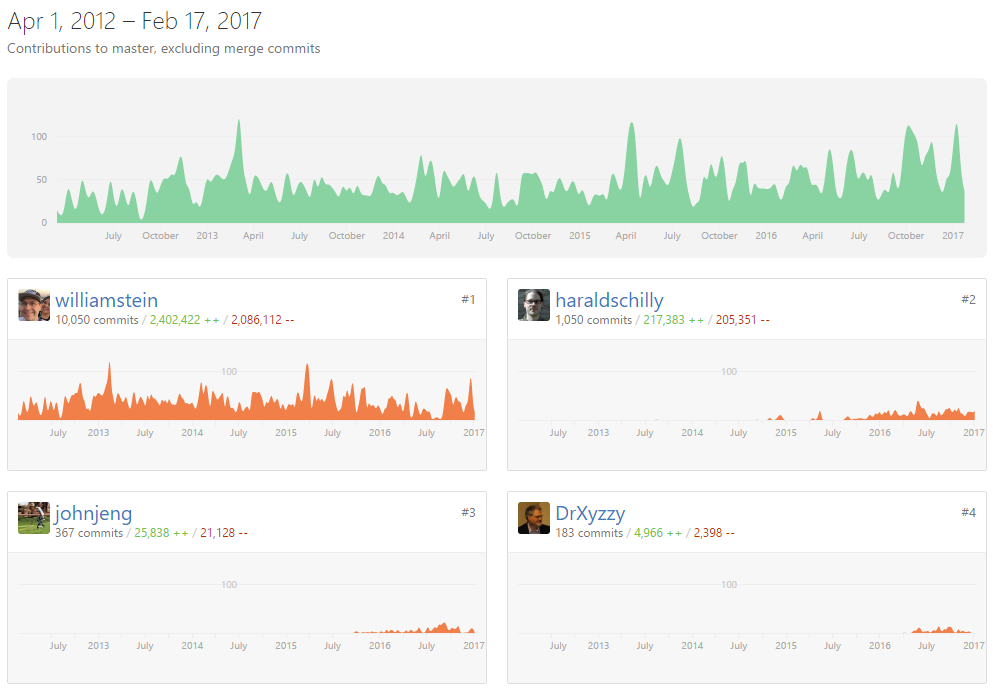
\includegraphics[width=\textwidth]{images/smc-contributions-2017-02-17.png}
\caption{top \SMC source contributors from the project's beginning in 2012 through February 2017}
\end{figure}

\section{Current state of \SMC's source code and documentation}

%% Summarize the current state of the source code, the current state of the
%% architecture documentation, and of the development documentation and
%% resources.  This is really "where the work started from".
\SMC's source code currently resides in a single \git repository hosted on
\GitHub.  This repository contains all code written uniquely for SMC--web-based
frontend and all backend servers--as well as scripts and tools for development
of SMC.

It also has a collection of many small scripts and utilities used for managing
the live SMC site and the many servers that comprise it (hubs, compute nodes,
etc.)  Many of these are just single command-line commands for what might be
common tasks.  Though there is no documentation for most of these tools or when
and how they should be used.  Most of them are not directly relevant to
doing development of SMC.

Most of the main SMC source code is split across two \Python packages, five
\JavaScript, and one directory containing additional web resources such as
fonts and images, as well as "vendored" \JavaScript--third-party source code
that may require special handling to integrate into the SMC web app.

There is also a configuration script for Webpack,
%% Reference link to webpack here %%
a tool used to bundle \JavaScript sources, HTML, images, and other resources
into a working website.  This file serves as something of a map to how all of
SMC's frontend code fits together.  Because there is no equivalent for the
backend, it is a little more difficult at first to understand how the
server-side code works.  That said, the general layout is clear enough that an
experienced developer, armed with high-level documentation of SMC's
infrastructure, can gain insight into what features might be implemented where.
More such high-level documentation is needed, however.

Beyond a few brief "README" files in the main source packages, and scattered
in-line documentation in some of the source files, there is very little
documentation of what each source file is or what internal or external APIs
might exist.  So while the high-level structure is not difficult to understand,
it is somewhat more difficult to understand the flow of data and program
control.

\section{Overview of \SMC's internal design}

%% Provide a brief summary of my documentation of SMC's internals, with link
%% to the full documentation.  Explain how this should help others understand
%% how SMC works, even given its relative flux.  Discuss future work needed
%% to understand the source code and its modularization.

\section{Overview of \SMC's software development process}
%% Summarize work done improving development processes and explain ongoing
%% and future work needed in this area.

\section{Conclusion and future work}
%% Conclude with summary of where we started, where we are now, and what work
%% is still needed.  Perhaps raise open questions about whether or not D3.4, as
%% currently documented in the proposal, is worth pursuing, and why/why not.


\printbibliography
\end{document}

%%% Local Variables:
%%% mode: latex
%%% TeX-master: t
%%% End:

%  LocalWords:  githubissuedescription newpage tableofcontents newpage printbibliography
